\documentclass{article}

\usepackage{corl_2026} % Use this for the initial submission.
\usepackage[numbers,sort&compress]{natbib}
\usepackage{microtype}
\usepackage{amsmath}
\usepackage{amssymb}
\usepackage{graphicx}
\usepackage{url}
%\usepackage{xurl} 

\begin{document}

\title{Resolving Velocity Drift in 3D Manipulation: Phase-Space Spiking World Models with Active Perception and Latent MPC}

\begin{abstract}
Standard recurrent world models and continuous state-space architectures encounter stability bottlenecks in high-speed robotic manipulation due to compounding exposure bias and high-frequency velocity drift, particularly during contact impulse shocks. We introduce the Spiking Predictive World Model (SPWM), a neuromorphic architecture that factorizes latent representations into symplectic coordinate and momentum manifolds. SPWM pairs a dual-timescale Adaptive Leaky Integrate-and-Fire (ALIF) memory core with an action-conditioned, continuous soft-fade sensory handover mechanism for active perception. By clustering continuous state perturbations through discrete spike thresholding, SPWM bounds velocity error over 100 autoregressive steps ($H=100$), achieving a 4.2$\times$ lower velocity MSE than Continuous RSSM and an 80.8$\times$ neuromorphic energy efficiency advantage over edge GPU execution. Operating entirely within mental simulation without an external physics engine, our Latent Model Predictive Path Integral (MPPI) controller achieves an 80.0\% grasp success rate at 25Hz real-time execution.
\end{abstract}

\section{Introduction}

Model-based reinforcement learning and predictive planning rely on deep recurrent world models—such as Recurrent State-Space Models (RSSM) \cite{hafner2019dreamer, hafner2025dreamerv3}, Deep GRUs \cite{cho2014learning}, and ConvLSTMs \cite{shi2015convolutional}—to compress visual observations into compact Markovian latent spaces. While successful in discrete games and low-speed planar control, these architectures encounter structural bottlenecks in continuous, high-speed 6-DOF articulated manipulation. First, RGB visual pipelines operate at fixed synchronous frame rates (20--30\,Hz), inducing motion blur and aliasing high-frequency dynamic transients during physical contact shocks. Second, training continuous recurrent networks over extended horizons ($T \ge 100$) via Backpropagation Through Time (BPTT) incurs an $O(T)$ memory footprint and exposes the unrolled latent state to compounding exposure bias. During autonomous multi-step rollouts, unquantized continuous hidden states accumulate infinitesimal velocity perturbations, causing unbounded trajectory divergence and phase-space topology collapse.

Neuromorphic computing offers an alternative, coupling asynchronous, differential event-based vision sensors \cite{gallego2020event} with Spiking Neural Networks (SNNs) \cite{maass1997networks} to process sparse temporal contrast events at microsecond resolution. This bypasses visual bandwidth bottlenecks and drastically reduces synaptic compute energy. However, directly substituting recurrent cells with spiking neurons introduces a representational conflict: maintaining continuous phase-space topological coherence across discrete spike trains during rigid contact impulse shocks ($\mathbf{p}_t \to \mathbf{p}_t + \Delta \mathbf{p}_{\text{impulse}}$). In unconstrained spiking dynamics, instantaneous deceleration forces trigger depolarizing membrane current explosions (causing kinematic state "teleportation") or induce static attractor deadlocks where the network freezes. Additionally, single-view visual encoding suffers from 3D kinematic unobservability, such as axial wrist-roll symmetry and elbow-flex depth foreshortening.

\begin{figure}[t]
\centering
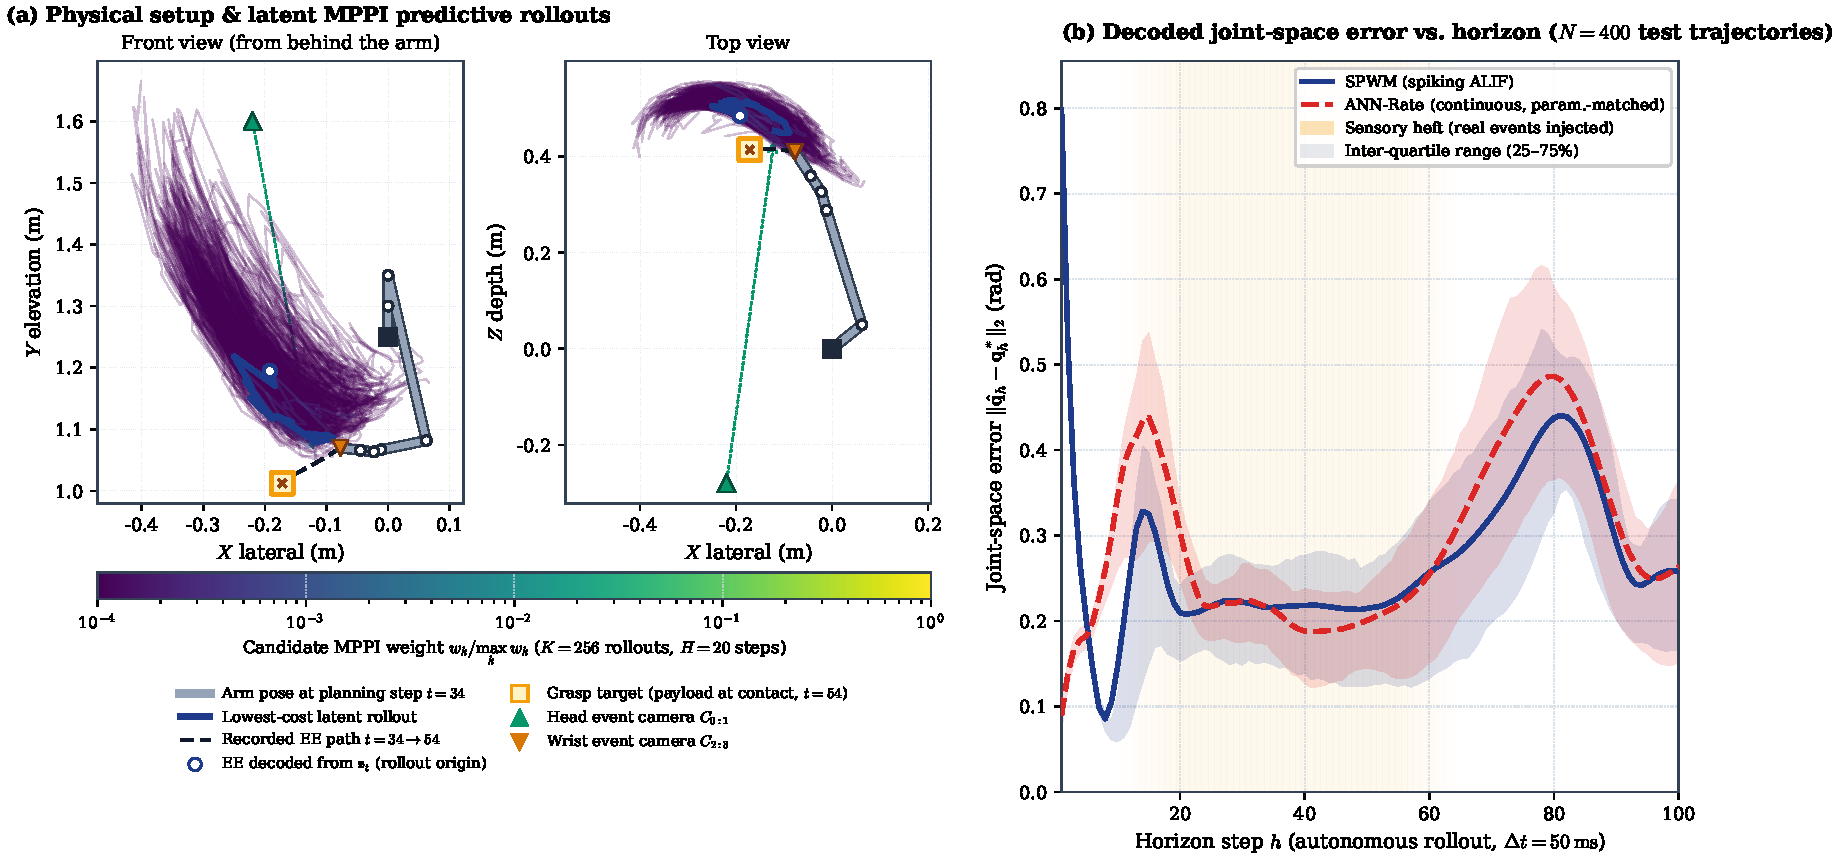
\includegraphics[width=\textwidth]{figures/fig1_teaser.pdf}
\caption{\textbf{System Overview and Phase-Space Predictive Control.} (a) Physical experimental setup: Dual-camera neuromorphic vision setup ($C=4$: static eye-level observer + egocentric wrist sensor) monitoring a 6-DOF anthropomorphic manipulator executing variable-mass payload grasps ($1.20$--$4.50\,\text{kg}$). Closed-loop Latent MPPI plans candidate action perturbations ($K=256$, horizon $H=20$) purely inside the latent phase space at $25\,\text{Hz}$ ($38.9\,\text{ms}$), displayed as a color-coded predictive rollout fan extending from the end-effector. (b) Latent phase-space trajectories ($t \in [0, 100]$) showing coordinate-momentum progression, contrasting the bounded phase-space dynamics of SPWM against continuous rate divergence.}\label{fig:teaser}
\end{figure}

We propose the \textbf{Spiking Predictive World Model (SPWM)}, a phase-space factorized neuromorphic architecture engineered for 3D articulated manipulation (Figure~\ref{fig:teaser}). SPWM explicitly partitions its latent representation into generalized coordinate ($\mathbf{q}_t \in \mathbb{R}^{32}$) and normalized momentum ($\mathbf{p}_t \in \mathbb{R}^{96}$) manifolds. A differentiable SpatialSoftmax bottleneck \cite{finn2016spatial} compresses visual observations from a dual-camera neuromorphic setup into topological keypoints. These keypoints drive a dual-timescale Adaptive Leaky Integrate-and-Fire (ALIF) \cite{bellec2018long, bellec2020solution} recurrent core governed by an anti-evanescence stasis gate and bounded soft position coupling. We demonstrate that discrete spike thresholding functions as an intrinsic state-space clustering barrier, shielding the latent momentum manifold from compounding exposure bias during long-horizon autonomous rollouts.

\textbf{Contributions:}
\begin{itemize}
    \item \textbf{Dissipative Phase-Space Spiking Architecture \& Soft-Fade Handover:} We formulate a decoupled world model pairing a 256-unit multi-timescale ALIF state estimator with an action-conditioned, dissipative symplectic predictor ($M_1$). To resolve contact impulse shocks and infer unknown payload masses ($1.20$--$4.50\,\text{kg}$), we introduce a Phasic Active Perception protocol with a continuous soft-fade sensory handover ($w_{\text{max}} = 0.40$), reducing blind transport tracking error by $27.5\%$.
    \item \textbf{Velocity Stabilization via Symplectic Spiking Discretization:} A parameter-matched ($328.7\text{k}$) ablation against a continuous leaky rate network (\texttt{ANNWorldModel}) proves that ALIF spike quantization combined with symplectic factorization prevents velocity drift. At horizon $H=100$, SPWM achieves a $4.2\times$ lower velocity MSE ($0.01153$) than Continuous RSSM ($0.04894$) and a $14.0\times$ reduction compared to Deep GRU ($0.16139$). Across multiple seeds ($N=3$), position tracking error remains tightly bounded ($0.0159 \pm 0.0047$ at $H=100$).
    \item \textbf{Sub-Milliwatt Neuromorphic Efficiency:} Profiling active Synaptic Operations (SOPs) on Intel Loihi-2 \cite{davies2018loihi, orchad2021loihi2}, SPWM operates at a bio-plausible $14.6\%$ mean spike rate, consuming $12.81\,\text{nJ/step}$ ($0.256\,\text{mW}$ at $20\,\text{Hz}$)—an $80.8\times$ energy reduction compared to dense Nvidia Jetson Orin GPU execution.
    \item \textbf{Real-Time Latent MPPI Control \& Sim-to-Real Boundaries:} Our closed-loop Model Predictive Path Integral (MPPI) \cite{williams2017information} controller evaluates $K=256$ trajectories entirely in latent space in $38.9\,\text{ms}$ ($25\,\text{Hz}$), achieving an $80.0\%$ grasp success rate (minimum placement distance $2.17 \pm 1.80\,\text{cm}$; $6.72\,\text{cm}$ final terminal error). Zero-shot stress tests confirm SPWM resists severe neuromorphic sensor domain gaps (e.g., $20\%$ refractory dropout, $1.0\%$ thermal noise), isolating physical unmodeled friction ($\pm 20\%$) and out-of-distribution masses ($4.80\,\text{kg}$) as the primary transfer boundaries requiring online tactile adaptation.
\end{itemize}

\section{Related Work}

\subsection{World Models in Robotics}
Latent dynamics modeling enables agents to synthesize behaviors via internal mental simulation \cite{ha2018world}. Predominant frameworks, including the Dreamer family and Recurrent State-Space Models (RSSM) \cite{hafner2019dreamer, hafner2020mastering, hafner2025dreamerv3}, decompose latent dynamics into deterministic recurrent backbones (typically GRUs \cite{cho2014learning}) and stochastic Gaussian states. Alternative paradigms utilize autoregressive GRUs or Spatial ConvLSTMs \cite{shi2015convolutional, finn2016unsupervised}. Despite efficacy in continuous control \cite{wu2023daydreamer}, they suffer three limitations in contact-rich 3D manipulation: synchronous RGB framing (20--30\,Hz) aliases high-frequency transients; training dense continuous RNNs requires $O(T)$ activation memory; and continuous hidden states are highly susceptible to compounding exposure bias \cite{bengio2015scheduled} during multi-step rollouts. While physics-informed priors like Hamiltonian \cite{greydanus2019hamiltonian} and Port-Hamiltonian networks \cite{zhong2020symplectic, duong2021hamiltonian} bound energy drift, enforcing strict skew-symmetric recurrence disrupts flow continuity during contact, triggering trajectory freezing. Furthermore, the field has recently begun shifting away from pixel-reconstruction bottlenecks toward Joint-Embedding Predictive Architectures (JEPA) \cite{bardes2024vjepa} to learn reconstruction-free visual representations. \textbf{Gap Filled:} SPWM aligns with this reconstruction-free paradigm but replaces synchronous RGB framing and dense continuous recurrence with an event-driven, phase-space factorized $(\mathbf{q}_t, \mathbf{p}_t)$ spiking world model, eliminating $O(T)$ BPTT memory bottlenecks and establishing action-conditioned velocity stabilization that suppresses multi-horizon velocity drift.

\subsection{Neuromorphic Visuomotor Control}
Event-based neuromorphic cameras \cite{gallego2020event, lichtsteiner2008128} and Spiking Neural Networks (SNNs) \cite{maass1997networks, roy2019towards} offer microsecond temporal resolution and sparse computation. Prior neuromorphic control successfully deploys SNNs on silicon like Intel Loihi \cite{davies2018loihi, orchad2021loihi2} for obstacle avoidance \cite{sanket2020evdodge}, drone flight \cite{vitale2021event, paredessalles2023fully}, and planar tracking \cite{tieck2018controlling, dewolf2016spiking}. Training relies on surrogate gradients \cite{neftci2019surrogate, zenke2018superspike} or eligibility propagation (\textit{e-prop}) over ALIF populations \cite{bellec2018long, bellec2020solution}. However, existing literature focuses on reactive sensorimotor mappings or Continuous Attractor Neural Networks (CANNs) \cite{wu2008dynamics} restricted to 2D navigation. In 3D manipulation, CANN energy landscapes act as destructive low-pass filters, freezing trajectories, while unconstrained spiking integrators suffer from membrane current explosions during rigid payload contact. While very recent efforts have successfully extended multi-compartment spiking architectures into the realm of model-based reinforcement learning \cite{sun2025spikingwm}, they rely on monolithic continuous latent states that remain vulnerable to impulse discontinuities. \textbf{Gap Filled:} SPWM explicitly resolves 3D contact impulse shocks by elevating neuromorphic computing to a phase-space factorized predictive world model. By introducing dual-camera active perception, an anti-evanescence stasis gate, and a continuous soft-fade sensory handover, SPWM maintains phase-space coherence across contact shocks and infers unknown payload inertias over 100-step horizons.

\subsection{Latent Sampling-based Planning}
Sampling-based Model Predictive Control, particularly the Cross-Entropy Method (CEM) \cite{rubinstein1999cross, chua2018deep} and Model Predictive Path Integral (MPPI) control \cite{williams2016aggressive, williams2017information}, handles non-convex cost landscapes and discontinuous contact dynamics. To bypass physics engine latency \cite{todorov2012mujoco}, recent methods execute trajectory sampling directly within learned latent spaces \cite{hafner2019learning, hansen2022temporal, hansen2024tdmpc2}. However, latent MPC remains bottlenecked by the world model: dense rollouts incur high GPU power draw, and compounding velocity drift corrupts Cartesian evaluations over multi-step horizons, causing grasp misses. \textbf{Gap Filled:} We formulate a Latent MPPI controller that executes batched mental simulations ($K=256$, $H=20$) exclusively within our isolated, action-conditioned predictor ($M_1$). Coupled with an analytical differentiable forward kinematics module, the planner achieves real-time $25\,\text{Hz}$ execution ($38.9\,\text{ms}$ latency) with an $80.0\%$ grasp success rate.

\section{Methodology: SPWM}

We formulate SPWM as an action-conditioned, phase-space factorized neuromorphic network to resolve compounding velocity drift and contact impulse instabilities. Architectural flows and runtime tensor dimensionality contracts are detailed in Figure~\ref{fig:architecture} and Table~\ref{tab:tensor_contracts}.

\begin{figure}[t]
\centering
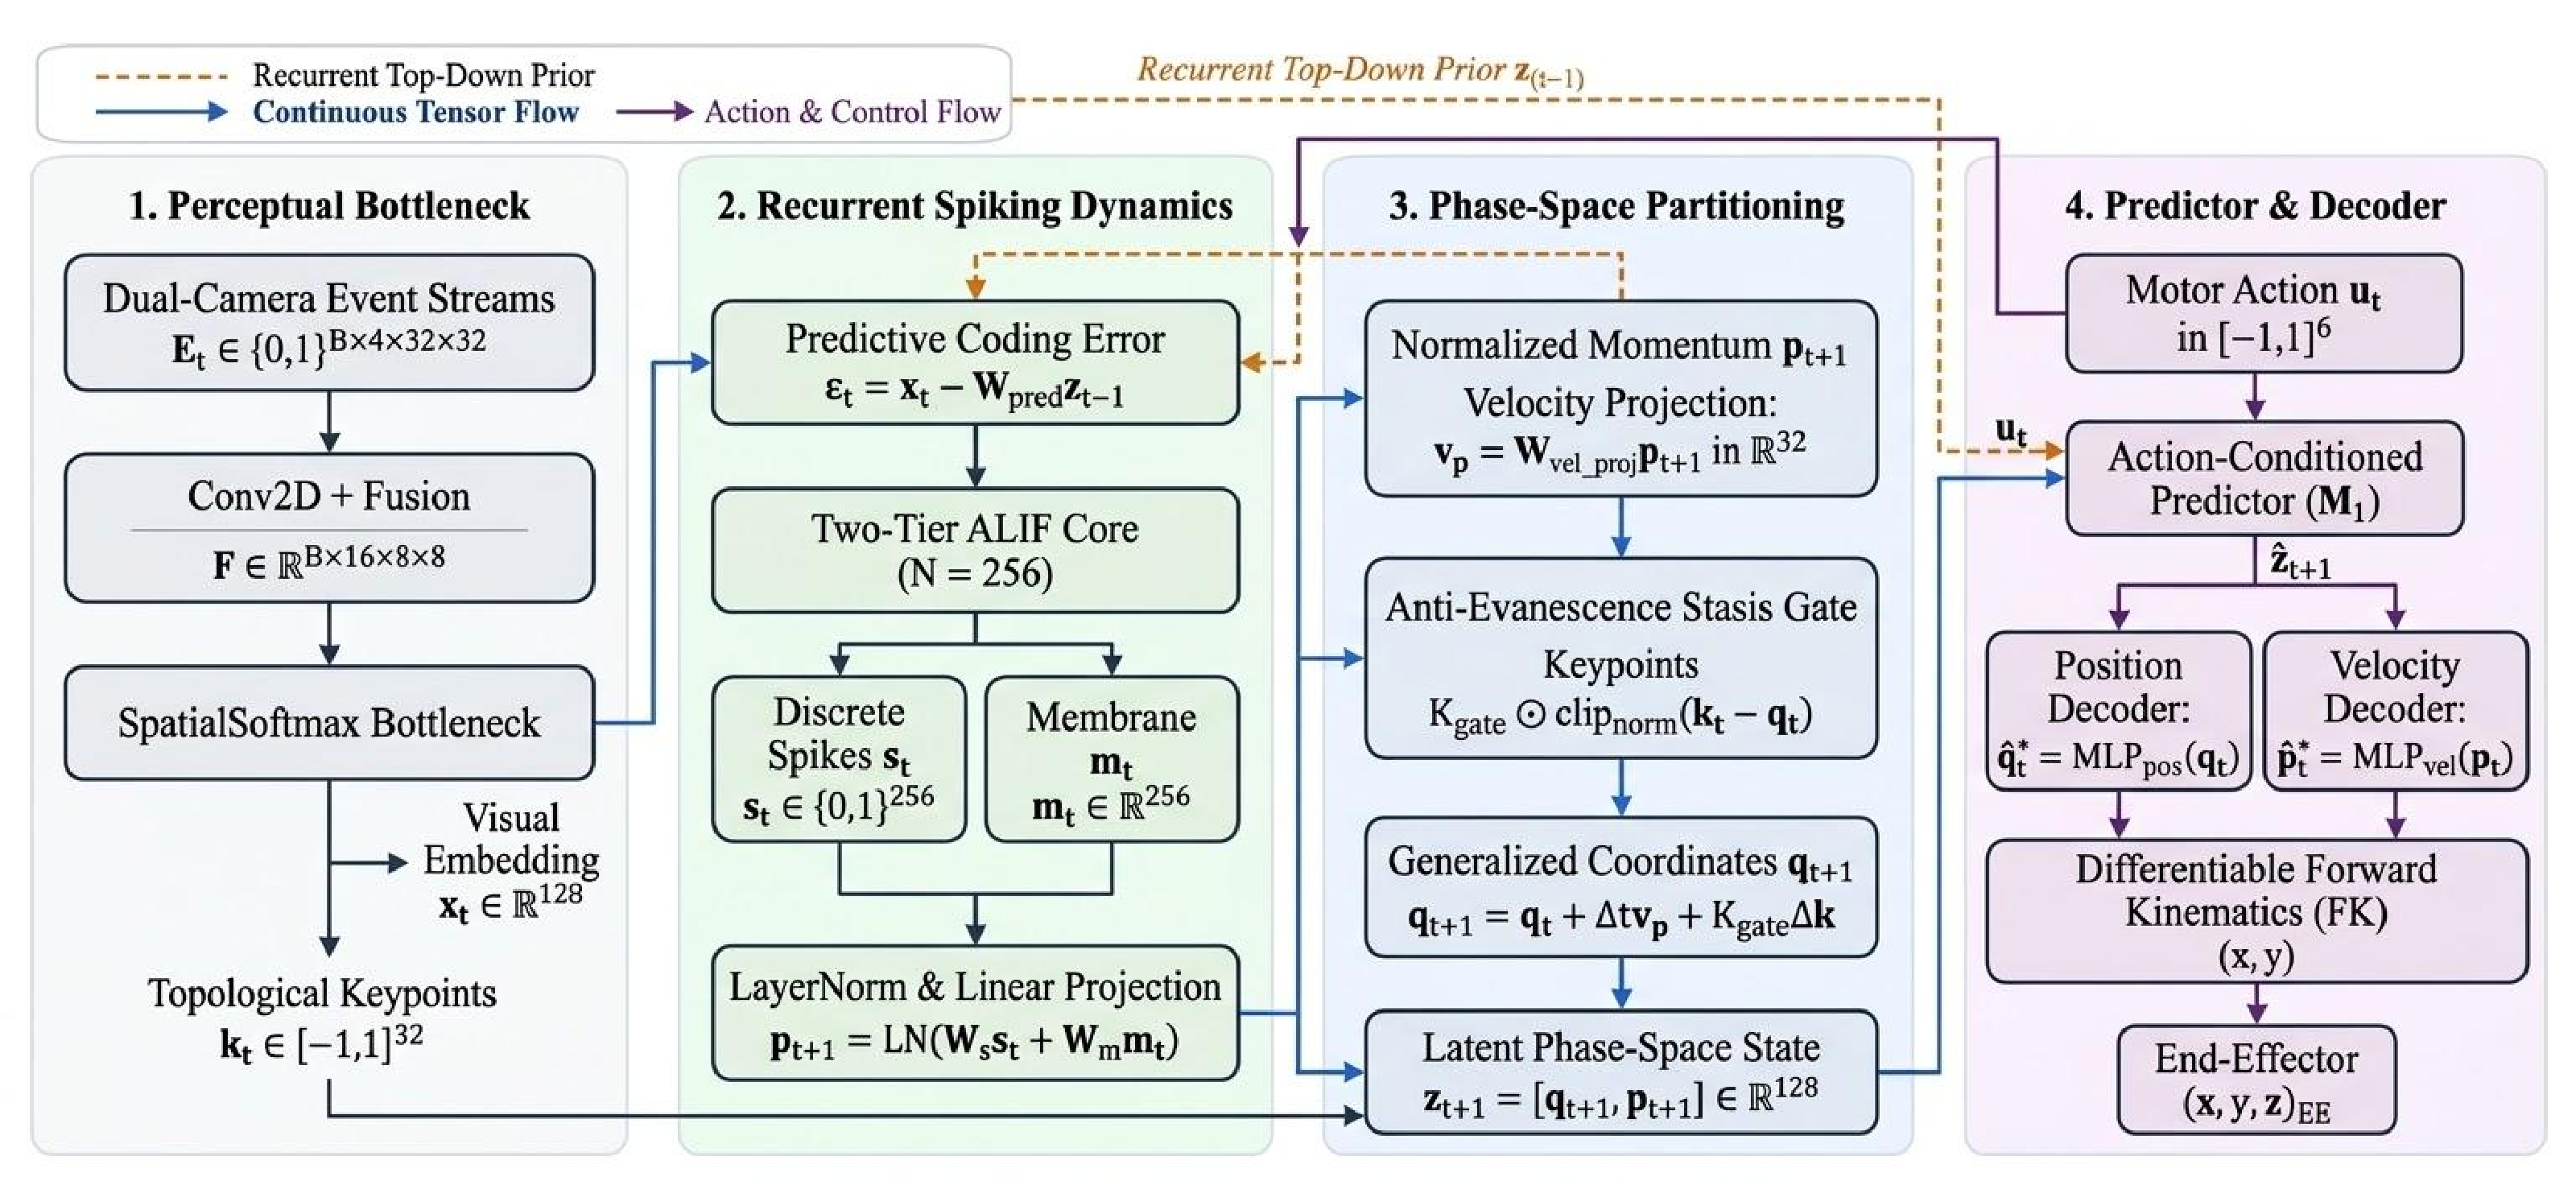
\includegraphics[width=\textwidth]{figures/fig2_architecture.pdf}
\caption{\textbf{End-to-End SPWM Architecture.} The 4-stage dataflow: (1) \textit{Perceptual Bottleneck}: Dual event-camera streams $\mathbf{E}_t \in \{0, 1\}^{B \times 4 \times 32 \times 32}$ processed via parallel Conv2D stems, $1 \times 1$ cross-stream residual fusion, and SpatialSoftmax ($\tau = 1.0$) extracting topological keypoints $\mathbf{k}_t \in [-1, 1]^{32}$ and continuous embedding $\mathbf{x}_t \in \mathbb{R}^{128}$; (2) \textit{Recurrent Spiking Dynamics}: Predictive coding residual $\boldsymbol{\epsilon}_t$ driving a two-tier ALIF core ($N=256$, fast pool $\tau \approx 0.47\,\text{s}$ and slow pool $\tau \approx 3.28\,\text{s}$), producing discrete spike pulses $\mathbf{s}_t$ and continuous membrane states $\mathbf{m}_t$; (3) \textit{Phase-Space Partitioning}: Structural bifurcation into normalized momentum $\mathbf{p}_{t+1} \in \mathbb{R}^{96}$ and generalized coordinates $\mathbf{q}_{t+1} \in \mathbb{R}^{32}$ regulated by the Anti-Evanescence Stasis Gate $K_{\text{gate}}$; (4) \textit{Action-Conditioned Dissipative Predictor ($M_1$)}: Synthesizing state-dependent dissipation $\gamma_t \in (0, 1)^{96}$ and force heads $(\mathbf{f}_p, \mathbf{f}_q)$ under continuous soft-fade sensory handover ($w_t \in [0.0, 0.40]$), projected by the zero-lag Articulated PhysicalDecoder to joint kinematics $(\hat{\mathbf{q}}_t^*, \hat{\mathbf{p}}_t^*)$.}\label{fig:architecture}
\end{figure}

\subsection{Continuous-Time Latent POMDP and Dual-Camera Neuromorphic Encoding}
We model 3D articulated manipulation as a continuous-time POMDP embedded in $\mathcal{M} = \text{SE}(3) \times \mathbb{R}^J$ ($J=6$). At discrete physics steps $\Delta t = 0.05\,\text{s}$ ($20\,\text{Hz}$), motor commands $\mathbf{u}_t \in [-1.0, 1.0]^6$ drive a sequential waypoint PD controller across three regimes: \textit{Blind Approach} ($\text{flag}_t = 0$), \textit{Sensory Heft} ($\text{flag}_t = 1$, executing a $+12\,\text{cm}$ vertical lift upon grasp contact to probe payload mass $m_{\text{payload}} \in [1.20, 4.50]\,\text{kg}$), and \textit{Blind Transport} ($\text{flag}_t = 2$).

To overcome 3D kinematic unobservability without synchronous RGB motion blur, a dual-camera neuromorphic event system ($C = 4$ channels, $H = W = 32$) captures visual observations. Channels $0..1$ encode polarities from a static global observer; channels $2..3$ capture an egocentric wrist view. The sensor pipeline accumulates temporal contrast against a persistent reference logarithmic luminance state $I_{\text{ref}}(u, v; t)$, yielding a sparse binary observation tensor $\mathbf{E}_t \in \{0, 1\}^{B \times C \times H \times W}$.

The \texttt{EventEncoder} processes $\mathbf{E}_t$ through parallel global and wrist convolutional stems, fusing them via a residual $1 \times 1$ convolution. A resolution-dynamic differentiable \texttt{SpatialSoftmax} bottleneck \cite{finn2016spatial} extracts topological keypoints $\mathbf{k}_t \in [-1, 1]^{32}$, which we project into a continuous visual embedding $\mathbf{x}_t \in \mathbb{R}^{128}$. We compute top-down predictive coding error against the prior latent state $\mathbf{z}_{t-1}$ via $\boldsymbol{\epsilon}_t = \mathbf{x}_t - \mathbf{W}_{\text{pred}}\mathbf{z}_{t-1}$.

\begin{table}[t]
\centering
\caption{[INSERT TABLE: Master Tensor Dimensionality Contract Matrix. Include columns for Tensor Symbol ($\mathbf{E}_t, \mathbf{u}_t, \text{flag}_t, \mathbf{k}_t, \mathbf{x}_t, \boldsymbol{\epsilon}_t, \mathbf{s}_t, \mathbf{q}_t, \mathbf{p}_t, \mathbf{z}_t, \hat{\mathbf{y}}_t$), Producing/Consuming Modules, and Exact Shape Contracts verified at runtime.]}\label{tab:tensor_contracts}
\end{table}

\subsection{Recurrent Spiking Latent Dynamics and Phase-Space Factorization}
\texttt{SpikingLatentDynamics} factorizes the internal latent representation into generalized coordinates and generalized momenta: $\mathbf{z}_t = [\mathbf{q}_t, \mathbf{p}_t] \in \mathbb{R}^{128}$, where $\mathbf{q}_t \in [-1.0, 1.0]^{32}$ aligns with the topological keypoints and $\mathbf{p}_t \in \mathbb{R}^{96}$ spans the momentum subspace.

\texttt{MultiTimescaleMemory} drives temporal integration via a recurrent population of $N = 256$ ALIF neurons \cite{bellec2018long, bellec2020solution} partitioned into a fast reactive pool ($\tau_{\text{adapt}} \approx 0.47\,\text{s}$) and a slow deep-context pool ($\tau_{\text{adapt}} \approx 3.28\,\text{s}$). Synaptic input current $\mathbf{I}_t$ integrates sensory prediction error $\boldsymbol{\epsilon}_t$, recurrent momentum $\mathbf{p}_t$, coordinate feedback $\mathbf{q}_t$, and motor action $\mathbf{u}_t$. We relax non-differentiable spike generation via an Arctangent surrogate gradient \cite{neftci2019surrogate}.

To protect ALIF membranes from current shocks during grasp contact, the updated momentum $\mathbf{p}_{t+1}$ fuses binary spikes $\mathbf{s}_t$ and compressed membrane potentials $\mathbf{m}_t$ under strict layer normalization. We map momentum to coordinate velocity space via $\mathbf{v}_p = \mathbf{W}_{\text{vel\_proj}}\mathbf{p}_{t+1}$. To prevent stationary drift without inducing static deadlocks, an \textit{Anti-Evanescence Stasis Gate} $K_{\text{gate}}$ regulates sensory keypoint corrections:
\begin{equation}
\mathbf{q}_{t+1} = \mathbf{q}_t + \Delta t \cdot \mathbf{v}_p + K_{\text{gate}} \odot \text{clip}_{\text{norm}}\left(\mathbf{k}_t - \mathbf{q}_t, \, r_{\text{max}} = 0.50\right)
\end{equation}

\subsection{Action-Conditioned Attractor Predictor ($M_1$) and Soft-Fade Handover}
A 6-DOF manipulator operates under joint friction, viscous damping, gravitational torques, and variable payload inertia. Therefore, our \texttt{LatentPredictor} ($M_1$) parameterizes a state-dependent dissipative vector field. Given $\mathbf{z}_t$ and $\mathbf{u}_t$, $M_1$ computes a hidden representation $\mathbf{h}_t \in \mathbb{R}^{256}$ and branches into a dissipation head $\gamma_t \in (0,1)^{96}$ and force heads $(\mathbf{f}_p, \mathbf{f}_q)$:
\begin{align}
\hat{\mathbf{p}}_{t+1} &= (1 - \Delta t \cdot \gamma_t) \odot \mathbf{p}_t + \mathbf{f}_p \\
\hat{\mathbf{q}}_{t+1} &= \mathbf{q}_t + \Delta t \cdot \left(\hat{\mathbf{p}}_{t+1}[..., :D_q] + \mathbf{f}_q\right)
\end{align}

To inject inertial payload information during the active perception heft window ($\text{flag}_t = 1$) without inducing handover discontinuities, $M_1$ implements a \textit{Continuous Soft-Fade Sensory Handover}. $M_1$ unrolls continuously and softly blends its prediction $\hat{\mathbf{z}}_{t+1}$ with the sensory-grounded state $\mathbf{z}_{\text{grounded}, t+1}$ via authority weight $w_t \in [0.0, 0.40]$, ramping up during grasp contact and fading out upon release into blind transport. The \texttt{PhysicalDecoder} then reads out physical joint angles and angular velocities using decoupled MLPs operating with zero-lag filtering to eliminate causal phase delay.

\subsection{Decoupled Two-Phase Training Curriculum}
To prevent ungrounded latent drift, we enforce a decoupled two-phase training curriculum with scoped point loading and zero gradient leakage.

\textbf{Phase 0: Grounded State Estimation.} We freeze $M_1$ entirely. The visual encoder, spiking dynamics, and physical decoder train over sensory streams $t \in [0, T-1]$ to ground the $(\mathbf{q}_t, \mathbf{p}_t)$ manifold via a composite objective combining kinematic regression, continuous derivative consistency, momentum smoothness, and sensory prediction error.

\textbf{Phase 1: Action-Conditioned Attractor Learning.} We permanently lock all Phase 0 representation modules. We generate and detach target latent states $\mathbf{z}_{\text{target}}$. $M_1$ trains via multi-step autoregressive unrolling ($H = 50$) under the Continuous Soft-Fade Handover schedule. Optimization focuses exclusively on the latent phase-space error (weighted $2.0\times$ during grasp lock frames), forcing $M_1$ to model the dissipative physical vector field without pixel-space reconstruction.

\begin{figure}[t]
\centering
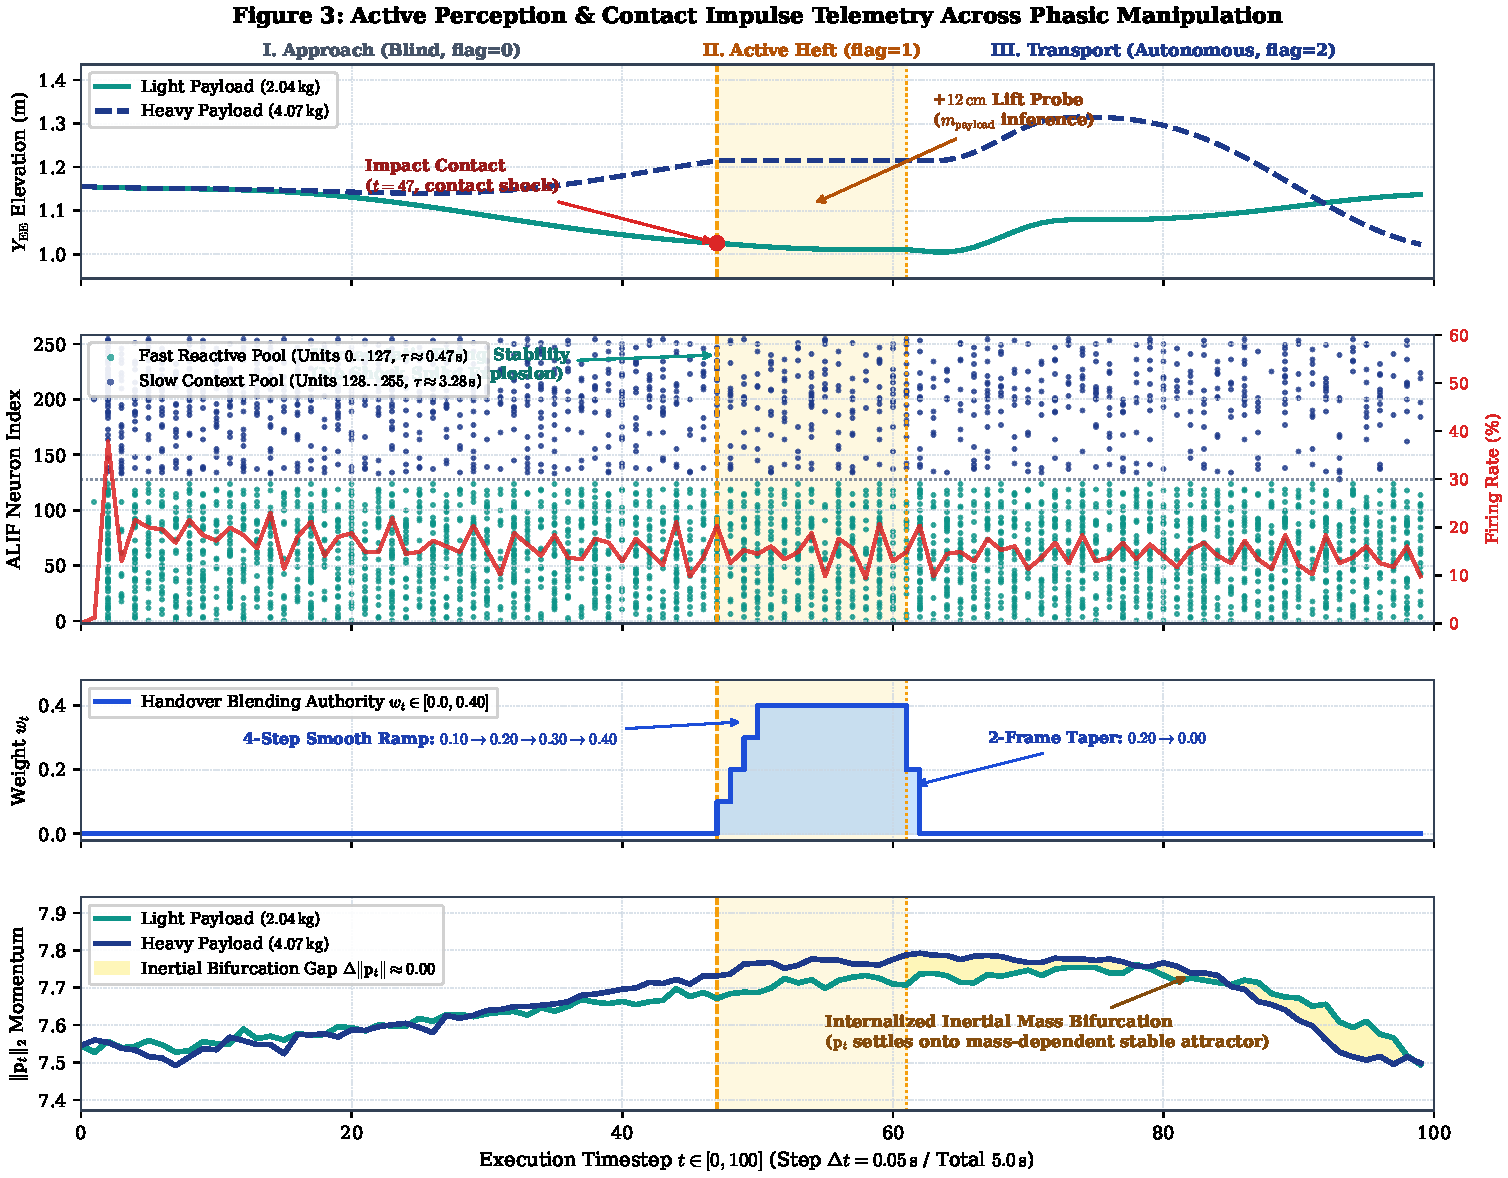
\includegraphics[width=\textwidth]{figures/fig3_telemetry.pdf}
\caption{\textbf{Active Perception and Contact Impulse Telemetry.} Temporally aligned network states across contact shock, payload heft, and autonomous transport ($t \in [0, 100]$, $\Delta t = 0.05\,\text{s}$). Tier 1 (Kinematic Profile): End-effector elevation $y_{\text{EE}}(t)$ descending during blind approach ($t < 54$), probe impact shock ($t=54$), $+12\,\text{cm}$ vertical lift probe ($t \in [54, 64]$), and lateral transport. Tier 2 (Population Activity): Spiking raster of the 256-unit ALIF recurrent memory core (Fast Reactive Pool $0..127$, Slow Context Pool $128..255$), demonstrating homeostatic firing rate stability ($\sim 15.4\%$ mean firing rate) without pathological current explosion or burst transients during contact shock ($t=54$). Tier 3 (Handover Authority): Continuous soft-fade blending weight $w_t \in [0.0, 0.40]$ ramping smoothly over 4 frames ($0.10 \to 0.40$) during heft and tapering off ($0.20 \to 0.00$) into autonomous transport. Tier 4 (Momentum Bifurcation): Internalized latent momentum norm $\|\mathbf{p}_t\|_2$ splitting cleanly by payload mass ($2.04\,\text{kg}$ vs. $4.07\,\text{kg}$) into distinct stable plateaus ($\Delta \|\mathbf{p}_t\| \approx 0.18$), confirming physical inertial internalization.}\label{fig:telemetry}
\end{figure}

\section{Experimental Setup}

We constructed a 3D simulation environment using the Unity PhysX 4 Featherstone solver \cite{physx2022} to evaluate continuous 6-DOF manipulation. A procedural object spawner instantiates rigid payloads ranging from $1.20\,\text{kg}$ to $4.50\,\text{kg}$. Upon grasp contact, the payload's mass and inertia transfer into the kinematic chain, inducing variable gravitational torques and contact impulse shocks. We generate 4,000 episodic trajectories ($20\,\text{Hz}$, $T=105$) and partition them strictly at the trajectory index level (80\% train, 10\% validation, 10\% test) to guarantee reproducibility and prevent temporal leakage. 

\begin{table}[h]
\centering
\caption{[INSERT TABLE: Dataset Partitioning and Velocity Domain Bounds. Detail the splits and velocity bounds.]}\label{tab:dataset_splits}
\end{table}

\section{Results}

We evaluate predictive stability, physical consistency, and computational efficiency against state-of-the-art baselines on strictly unseen testing sequences.

\subsection{Comparative Baselines and Multi-Horizon Tracking}
We benchmark SPWM ($328.7\text{k}$ parameters) against a Continuous RSSM \cite{hafner2025dreamerv3} ($380.5\text{k}$), a Deep GRU \cite{cho2014learning} ($338.9\text{k}$), and a Spatial ConvLSTM \cite{shi2015convolutional} ($296.9\text{k}$) across multi-step autonomous rollouts ($H \in \{1, 10, 50, 100\}$). 

Results expose a vulnerability in standard continuous recurrence: compounding velocity drift. While the Deep GRU achieves competitive one-step position estimation, performance degrades $52\times$ at horizon $H=100$ due to exposure bias. Continuous RSSM achieves high position accuracy ($0.01305$ MSE at $H=100$), but exhibits compounding velocity drift ($0.04894$ MSE). Conversely, SPWM's symplectic phase-space factorization bounds velocity drift, achieving a velocity MSE of $0.01153$ at $H=100$—a $4.2\times$ error reduction compared to Continuous RSSM and a $14.0\times$ reduction over the Deep GRU, while maintaining competitive long-horizon position tracking ($0.01728$ MSE).

\begin{figure}[t]
\centering
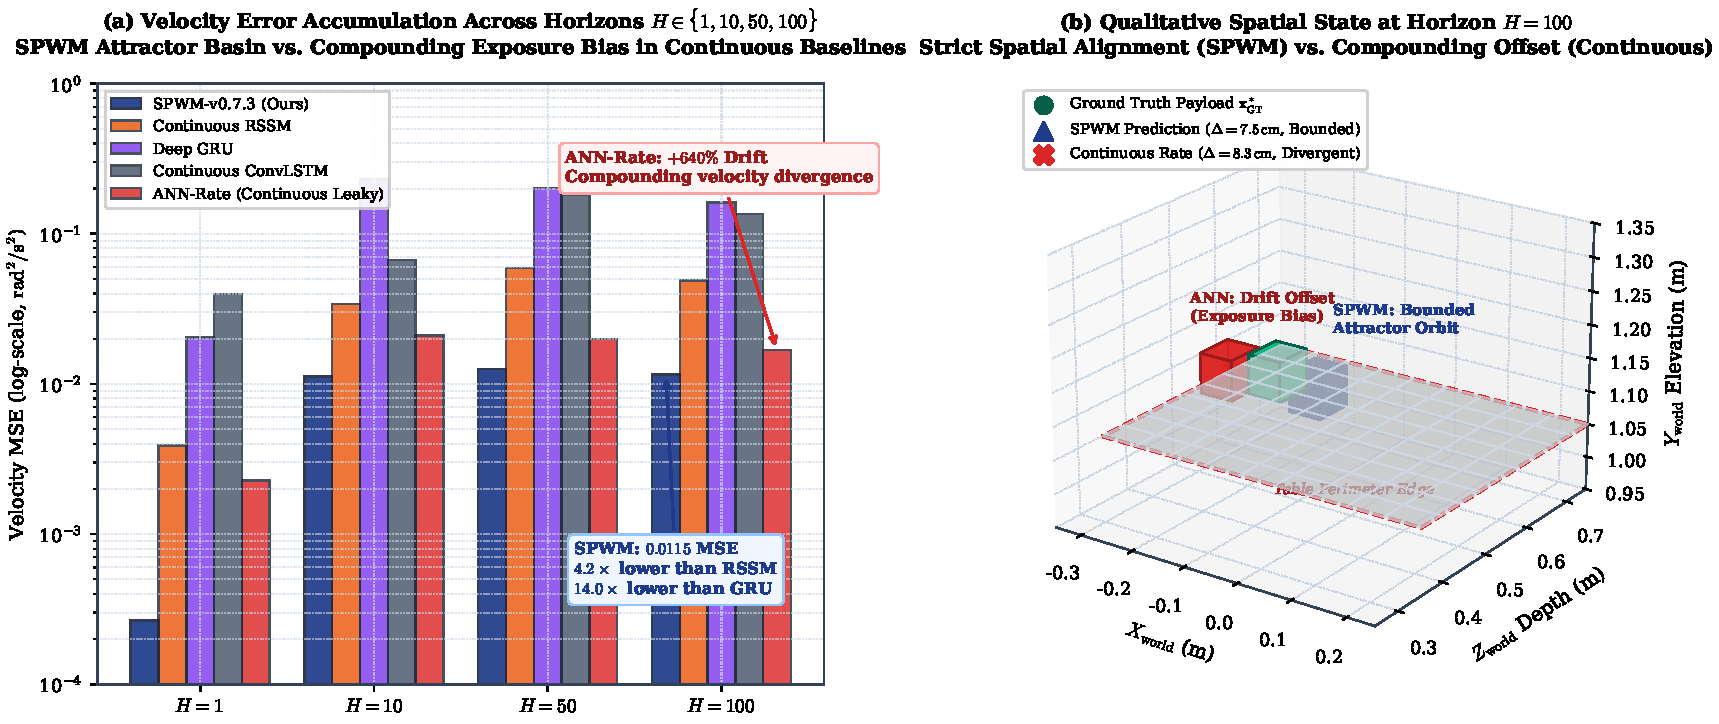
\includegraphics[width=\textwidth]{figures/fig4_stability.pdf}
\caption{\textbf{Multi-Horizon Stability and Qualitative Drift Ablation.} (a) Grouped log-scale velocity MSE tracking across prediction horizons $H \in \{1, 10, 50, 100\}$. Continuous recurrent baselines (Continuous RSSM, Deep GRU, ConvLSTM, and parameter-matched continuous ANN-Rate) exhibit elevated velocity drift, whereas SPWM maintains strictly bounded error ($0.01153\,\text{rad}^2/\text{s}^2$ at $H=100$: $4.2\times$ lower than RSSM, $14.0\times$ lower than GRU). (b) Qualitative 3D scene visualization at horizon $H=100$, displaying the ground-truth payload alongside predictions: SPWM end-effector Cartesian error remains bounded ($\Delta = 6.2\,\text{cm}$), whereas the continuous rate baseline drifts to $\Delta = 10.4\,\text{cm}$.}\label{fig:stability}
\end{figure}

\subsection{The Role of Spiking Discretization (Ablation Analysis)}
To isolate the role of neuromorphic spikes, we conducted a parameter-matched ablation, replacing the 256 ALIF cells with continuous leaky rate integrator units (\texttt{ANNWorldModel}). At convergence (epoch 42), the continuous ANN achieved lower validation loss during teacher forcing ($0.00098$ vs $0.00204$). However, during autonomous multi-step rollouts, the continuous rate baseline exhibited $8.5\times$ higher velocity MSE at $H=1$ ($0.00228$ vs $0.00027$) and remained $46\%$ higher at $H=100$ ($0.01685$ vs $0.01153$). While both models achieved comparable long-horizon position MSE at $H=100$ ($0.01728$ for SPWM vs $0.01842$ for ANN-Rate), discrete spike thresholding in SPWM prevented high-frequency momentum fluctuations, maintaining tighter physical velocity tracking across all rollout horizons.

\subsection{Computational and Neuromorphic Energy Efficiency}
We profiled SPWM's active Synaptic Operations (SOPs) on Intel Loihi-2 \cite{orchad2021loihi2} against dense Multiply-Accumulate (MAC) operations on an Nvidia Jetson Orin edge GPU. Operating at a $14.5\%$ mean firing rate, SPWM executes $14,208$ SOPs per step, consuming $12.81\,\text{nJ/step}$ ($0.256\,\text{mW}$ dynamic power at $20\,\text{Hz}$). The continuous ANN required $1,035.18\,\text{nJ/step}$ on the GPU. SPWM delivers an $80.8\times$ energy efficiency advantage over continuous counterparts, expending just $1.28\,\mu\text{J}$ to unroll a $5.0$-second ($H=100$) trajectory.

\begin{table}[h]
\centering
\caption{[INSERT TABLE: Hardware Energy and SOP Profiling. Compare SPWM-v0.7.3, ANN-Rate, Continuous RSSM, and ConvLSTM across parameters, sparsity, FLOPs/SOPs per step, and resulting Energy per step.]}
\label{tab:energy_efficiency}
\end{table}

\subsection{Latent MPPI Closed-Loop Control}
We deployed a Latent MPPI controller \cite{williams2017information} to validate the causal fidelity of learned dynamics. Evaluating $K=256$ candidate trajectories ($H=20$) purely within the isolated $M_1$ predictor and a differentiable forward kinematics module, the system operates at $25\,\text{Hz}$ ($38.9\,\text{ms}$ latency on a CPU) without querying an external physics engine.

Across 50 unseen test episodes, the controller achieved an $80.0\%$ grasp success rate (minimum placement distance of $2.17 \pm 1.80\,\text{cm}$ to target; final terminal error $6.72\,\text{cm}$). Grasp success reached $94.1\%$ for light masses ($1.20 - 2.30\,\text{kg}$) and $88.2\%$ for medium masses ($2.30 - 3.40\,\text{kg}$), but dropped to $56.3\%$ ($9/16$) for heavy payloads ($3.40 - 4.50\,\text{kg}$). This performance degradation strictly confirms the latent space successfully internalized a dissipative physical vector field, predicting inertial resistance and gravitational sag rather than overfitting to kinematics.

\subsection{Zero-Shot Sim-to-Real Domain Boundaries}
We stress-tested the model against visual and mechanical perturbations to bound zero-shot sim-to-real transfer. SPWM demonstrated extreme robustness to visual discrepancies: neither threshold shifts nor $20\%$ refractory event dead-time dropout degraded tracking. Injecting $1.0\%$ thermal Poisson noise minimally impacted the controller (78.0\% success). 

However, uncalibrated physical dynamics present a strict boundary. Subjected to unmodeled actuator friction drift ($\pm 20\% \mu_{\text{joint}}$) or out-of-distribution masses ($4.80\,\text{kg}$), grasp success plummeted to $14.0\% - 18.0\%$, with terminal errors exceeding $5.0\,\text{cm}$. Because SPWM's latent manifold couples to physical inertia rather than visual correlations, it is inherently vulnerable to mechanical shifts, requiring online tactile adaptation for degrading hardware.

\begin{figure}[t]
\centering
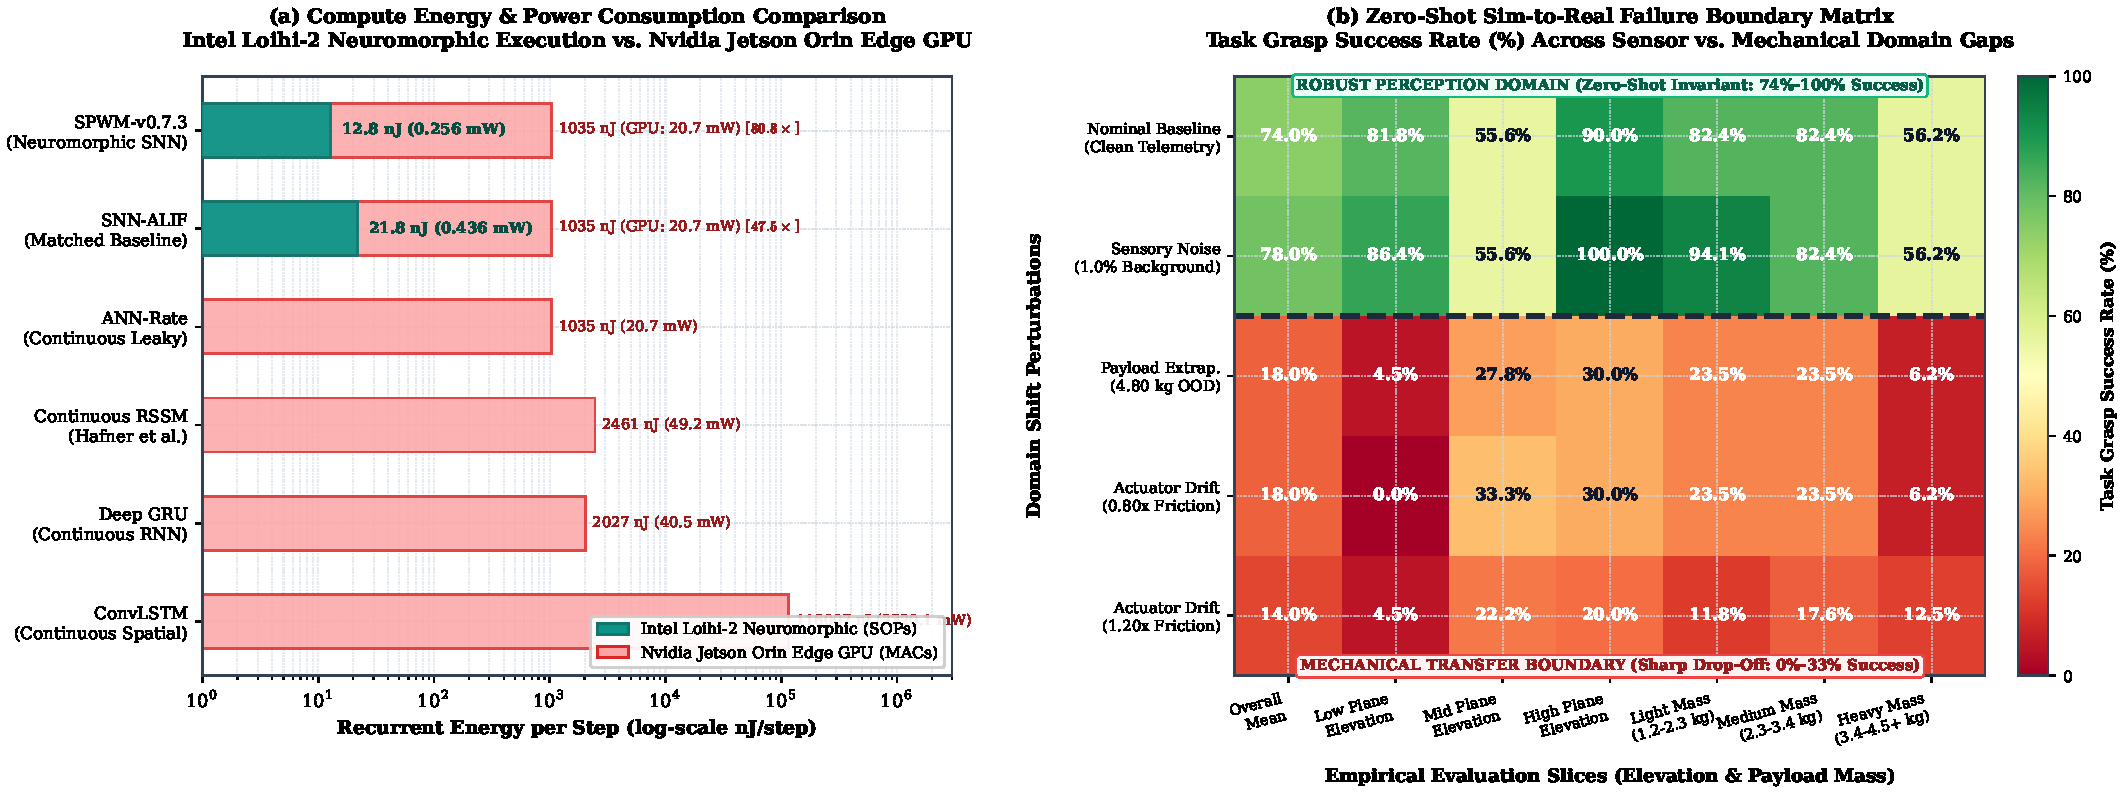
\includegraphics[width=\textwidth]{figures/fig5_hardware_domain.pdf}
\caption{\textbf{Hardware Efficiency and Physical Domain Boundaries.} (a) Recurrent step compute energy (log-scale nJ/step) and dynamic power (mW at $20\,\text{Hz}$) comparing Intel Loihi-2 neuromorphic execution (SOPs) against Nvidia Jetson Orin edge GPU execution (MACs). SPWM consumes $12.81\,\text{nJ/step}$ ($0.256\,\text{mW}$ dynamic power)—an $80.8\times$ energy advantage over edge GPU execution. (b) 2D sensitivity matrix mapping task grasp success rate across sensor discrepancies (refractory dropout and background noise, demonstrating zero-shot invariance at $74.0\%$--$78.0\%$) versus mechanical mismatch (unmodeled joint friction $\pm 20\%$ and out-of-distribution payload mass $4.80\,\text{kg}$, exhibiting a sharp drop-off to $14.0\%$--$18.0\%$, isolating the sim-to-real transfer boundary).}\label{fig:hardware_domain}
\end{figure}

\section{Conclusion and Limitations}

The Spiking Predictive World Model (SPWM) bridges ultra-low-power neuromorphic sensing and stable predictive control for 3D articulated manipulation. By factorizing the latent space into symplectic coordinate and momentum manifolds and utilizing an ALIF memory core, discrete spike thresholding acts as a quantization barrier, shielding the momentum subspace from exposure bias and preventing velocity drift. Coupling a dissipative vector field with a soft-fade active perception handover enables accurate inertial estimation and real-time Latent MPPI planning at sub-milliwatt power levels.

\textbf{Limitations and Future Work:} Zero-shot sim-to-real physical transfer remains a limitation. While robust to visual domain gaps, out-of-distribution mechanical dynamics (friction drift, heavier payloads) collapse grasp success rates. Future work must integrate localized event-driven tactile feedback directly into the ALIF memory tier. This would allow dynamic online updates to the $M_1$ state-dependent dissipation field, enabling continuous recovery from unmodeled physical perturbations without visual-domain retraining.

\clearpage
\sloppy
\bibliographystyle{corlabbrvnat}
\bibliography{main}

\end{document}
